% CREATED BY DAVID FRISK, 2016
\chapter{Theory}

\section{Project types}
When working on a project, it can be advantageous to identify what kind of project it starts off as. One model put forward by Obeng[SOURCE: Putting strategy to work, 1996] describes four project types. This is roughly the same model presented by Dombkins[?], which itself is a revised version of a model made by Turner \& Cochrane[?]. Instead of labeling them Type 1-4 or Type A-D, Obeng made the labels descriptive.

The project types each answer yes or no to the two questions: \textit{Is the project objective clear?} (or \textit{Is it known WHAT the project is?}) and \textit{Are the project methods clear?} (or \textit{Is it known HOW the project will be done?}).

\begin{table}[H]
\caption{Turner \& Cochrane, Dombkins and Obeng described the same type of project differently.}
\resizebox{\columnwidth}{!}{
\begin{tabular}{|c|c||c|c|c||c|}
\hline
& & \textbf{Turner \&} & & & \\
\textbf{What} & \textbf{How} & \textbf{Cochrane} & \textbf{Dombkins} & \textbf{Obeng} & \textbf{Example project} \\ \hline
yes & yes & Type 1 & Type A & Painting by NUMBERS & Engineering \\
yes & no & Type 2 & Type B & Going on a QUEST & Product development \\
no & yes & Type 3 & Type C & Making a MOVIE & Application development \\
no & no & Type 4 & Type D & Lost in a FOG & Research \\
\hline
\end{tabular}
}
\label{obengtable}
\end{table}

Obeng visualized these projects with a 2-by-2 matrix. Although the types are categorical, the axes are continuous. This means that a project can be represented by a point somewhere within the matrix.

\begin{figure}[H]
\hspace*{-1cm}
\centering
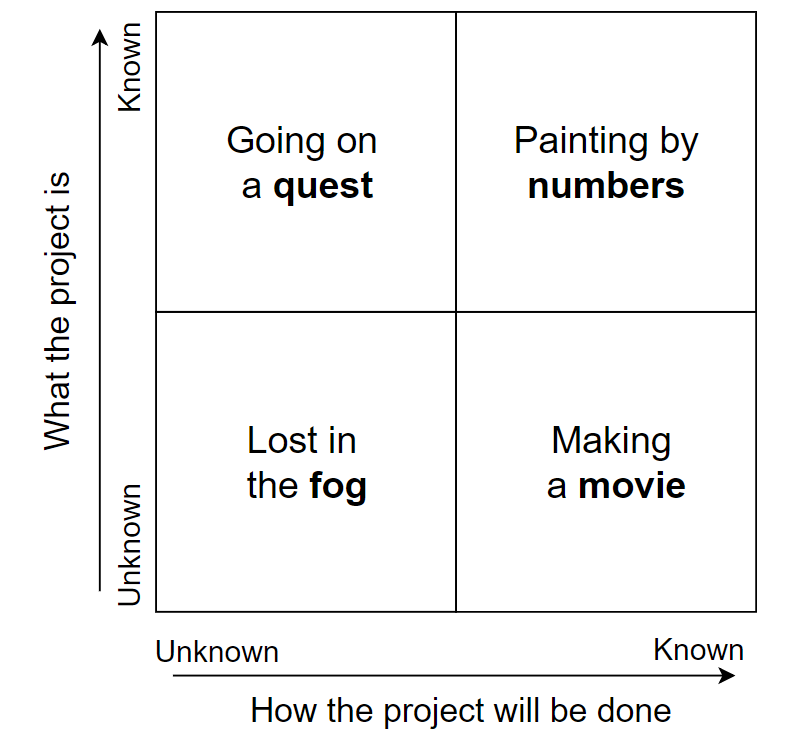
\includegraphics[scale=0.5]{figure/obeng1.png}
\caption{A redrawn illustration of Obeng's 4 project types.}
\label{obeng1}
\end{figure}

Robert Buttrick took Obeng's matrix further, introducing arrows to visualize that projects can change type as they progress. This is done by defining previously unknown HOWs and/or WHATs. [SOURCE ISBN:9780273745273].

\begin{figure}[H]
\hspace*{-1cm}
\centering
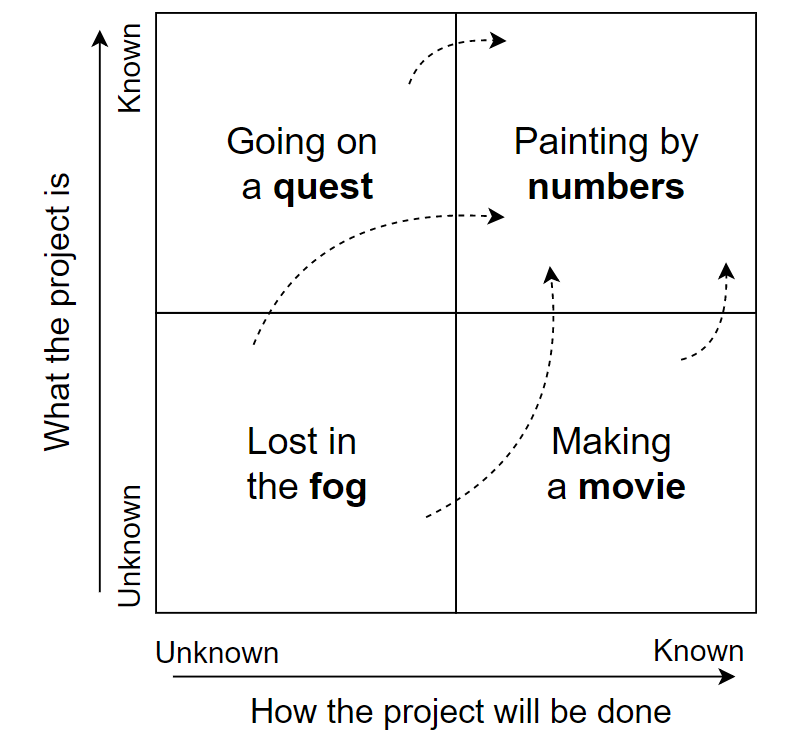
\includegraphics[scale=0.35]{figure/obeng2.png}
\caption{Projects usually resemble a NUMBERS-project more as they progress.}
\label{obeng2}
\end{figure}

Depending on the type of project, Obeng suggests differenent approaches to progressing them. If the WHATs and the HOWs are known, it gets easier to estimate the cost, time and result of a project. Conversely, a project with more unknowns requires work before it starts to look promising. The work required before projects with many unknowns show promise can vary, which is why Obeng recommends that at least the initial processes of these projects should follow an agile (iterative and/or parallell) methodology. Generally, projects closer to FOG benefit from agile methodology and projects closer to NUMBERS benefit from waterfall (linear) methodology.

\begin{figure}[H]
\hspace*{-1cm}
\centering
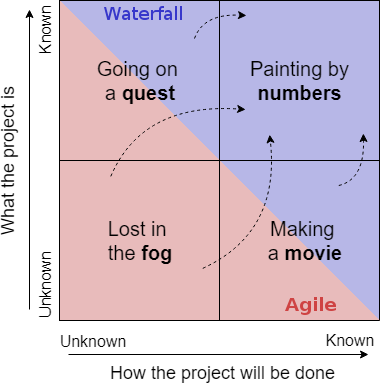
\includegraphics[scale=0.35]{figure/obeng3.png}
\caption{Projects closer to a NUMBERS-project benefit more from a waterfall methodology. Projects farther from a NUMBERS-project benefit more from agile methodology.}
\label{obeng3}
\end{figure}


\subsection{Types of teaching material projects}
It can be argued that designing teaching materials can start off as any type of project. 

One project may for example start with a set of inspirational resources, and the designer knows exactly what to add and what to remove to finish the project. The designer has a clear vision both concerning the WHATs and the HOWs of the project, making it a NUMBERS-project.

Another project may stem from a forced need of new teaching materials, because of a govermental decision to introduce programming in mathematics. The WHATs are somewhat known but if it is unknown how to reach these objectives, the project start off as a QUEST-project. If this project would be riddled with more question marks, for example if it would be unclear what programming language (if any) should be used and on what level the programming should to be taught, then the WHATs are less known and the problem would therefore start as a FOG-project.

Designing a teaching material as a MOVIE-project would be if the designer had all the skills (pedagogical, technological etc.) needed to create the teaching material, but did not know at the start of the project what content the teaching material should include or what objectives should be met.

\subsection{Types when revising teaching material projects}
When a teaching material has been created, more or less successfully, the teaching material can be used in a new project aiming to improve it. The teaching materials may not only change HOW the previous objectives are met, because it may sometimes prove beneficial to also change WHAT the objectives are. These projects therefore start as FOG-projects.



\section{Franklin's theory: Technology as a system} \label{franklintheory}
Since it is not obvious what the implications of shared teaching materials could be, it is important to stay critical and discuss the effects of certain material designs during the study. A certain perspective that can be used is one by U. Franklin, in the book and lecture series The Real World of Technology (Franklin, 1990). In it, she discusses technology as a complex system:

\begin{quote}
“Technology is not the sum of the artifacts, of the wheels and gears, of the rails and electronic transmitters. Technology is a system. It entails far more than its individual material components. Technology involves organization, procedures, symbols, new words, equations, and, most of all, a mindset. [...] Personally, I much prefer to think in terms not of systems but of a web of interactions. This allows me to see how stresses on one thread affect all others. The image also acknowledges the inherent strength of a web and recognizes the existence of patterns and designs.” - Franklin, 1990, pages 16 and 95.
\end{quote}

Since teaching materials encompass both a way of working and artifacts, they can be viewed as a technology, as defined by Franklin. As such, they affect how a teacher does their work in complex ways. For example, as Franklin also notes, materials can be used both to assist teachers in their lesson design, or to make them comply to certain standards and control structures. Therefore, it becomes important to consider effects on the teacher's work as a whole, instead of limiting the analysis to a specific lesson.

An important aspect of these systems of technology that Franklin defines is the difference between \textit{holistic} and \textit{prescriptive} technologies. In short, these can be described as the difference between an early industrial factory worker and an artisan: While the artisan maintains control over how they do their work throughout the whole production process, the factory worker works only on a specific task in a process controlled through strict social structures. The artisan relates to the holistic technology, while the factory worker relates to the prescriptive technology. Franklin further comments that, while prescriptive technology can be efficient and productive, it comes with a big social mortgage of a culture of compliance, and there only being one way of doing something.

%%%%%
\begin{comment} 
\section{Institutionalization}
\todo{The importance of institutionalization to our study need to be explained. Source: https://www.quora.com/What-is-political-institutionalization}
\begin{quote}
“Institutionalization, in this particular understanding -- needless to say there are others -- means that you set up a separate entity with the express delegated authority to do a thing.

Thereby the entity becomes the only proper Doing-a-thing-place. Doing the thing outside of the institution is either senseless (Playing chess without adhering to the rules of chess.) or will get you sanctioned. (Firing a gun outside of narrowly controlled circumstances.)“
\end{quote}
\end{comment}
%%%%%
\section{Krug's theory: What is usability, and how do you test it?}

Steve Krug is a usability consultant who wrote books about usability. His usability books are mainly focused on websites, but as he writes himself, his methods are applicable on other things as well.

Krug defines his first law of usability as \textit{“Don't make me think!“}, implying that users should understand what a website is and how to use it without expending any effort thinking about it:

\begin{quote}
“A person of average (or even below average) ability and experience can figure out how to use the thing to accomplish something without it being more trouble than it's worth.“ [SOURCE: DON'T MAKE ME THINK REVISITED, p.9]
\end{quote}

Aside from a few principles of usability, Krug puts a lot of effort into describing the usefulness of usability testing and how to do such testing in a cheap and easy manner. In his book specifically about usability testing, he defines such tests as:

\begin{quote}
“Watching people try to use what you're creating/designing/building (or something you've already created/desgined/built), with the intention of (a) making it easier for people to use or (b) proving that it is easy to use.“
\end{quote}

Or, in simpler terms:

\begin{quote}
“A facilitator sits in a room with the participant, gives him[/her] some tasks to do, and asks him[/her] to think out loud while he[/she] does them.“
\end{quote}

\subsection{Making usability testing scientific}

One important difference between Krug's method and the method used in this thesis is that Krug's focus is not to be scientific, but to merely improve what one is building [SOURCE: ROCKET SURGERY MADE EASY]. Thus, certain parts of his method have been adapted to make it easier to analyze:

\begin{enumerate}
	\item In contrast to Krug's method, the tasks in the tests are not altered mid-test. This makes them more comparable.
	\item There is more data gathering involved in the form of recordings and notes, rather than having a group of observers watching the test, to make analysis and comparison easier long after the tests have been conducted.
\end{enumerate}

\subsection{Connecting usability theory for websites to teaching materials}

One can argue that there is a large difference between teaching materials and websites. While in some cases these can be the same, such as online materials shared through a blog post, a teaching material can sometimes take the form of a book, a single PDF file, and more. All the materials have in common is that they are used to facilitate and/or empower a teacher's work. However, usability testing is still clearly applicable in the sense that it consists of observing someone using what you are testing.

Since teaching materials can be used in many different ways, the use case had to be narrowed down. Thus, in this thesis, the use case that the usability tests cover consist mainly of how teachers use teaching materials to plan their lessons. This does not mean that other use cases are ignored, such as a teacher simply using a material to learn more about a subject. However, the lesson planning is the main focus of the usability testing in this thesis.

\section{Adaptive Software Development}
The main method of collecting data for this study consisted of a process inspired by Adaptive Software Development (ASD). This method involves iterative development with strengths that fit this study, such as being flexible and low risk. This can for example mean that new information
can be easily adopted in future tests and that results can be delivered even if test subjects decide to terminate involvement in this study early. (Sommerville, 2016)

ASD is an antecedent to Agile Software Development, paving the way for popular project management methodologies such as Scrum and Kanban. The methodology for this study has no need of being as complex as Scrum or Kanban, one of the main reasons being the relative small size of the development team (i.e. the two authors of this paper), whereas for example the Scrum model is generally used by splitting a larger workforce in teams of 3 to 9. (Schwaber, 2004)

As can be seen in Figure~\ref{asd} ASD consists of three stages with a feedback loop, enabling developers to perform multiple iterations of improvement based on what they learn from users. This model is similar to the methodology that was developed in this study to collect data on usability of teaching materials. (Highsmith, 2000, p.84)


\begin{figure}[H]
\hspace*{-1cm}
\centering
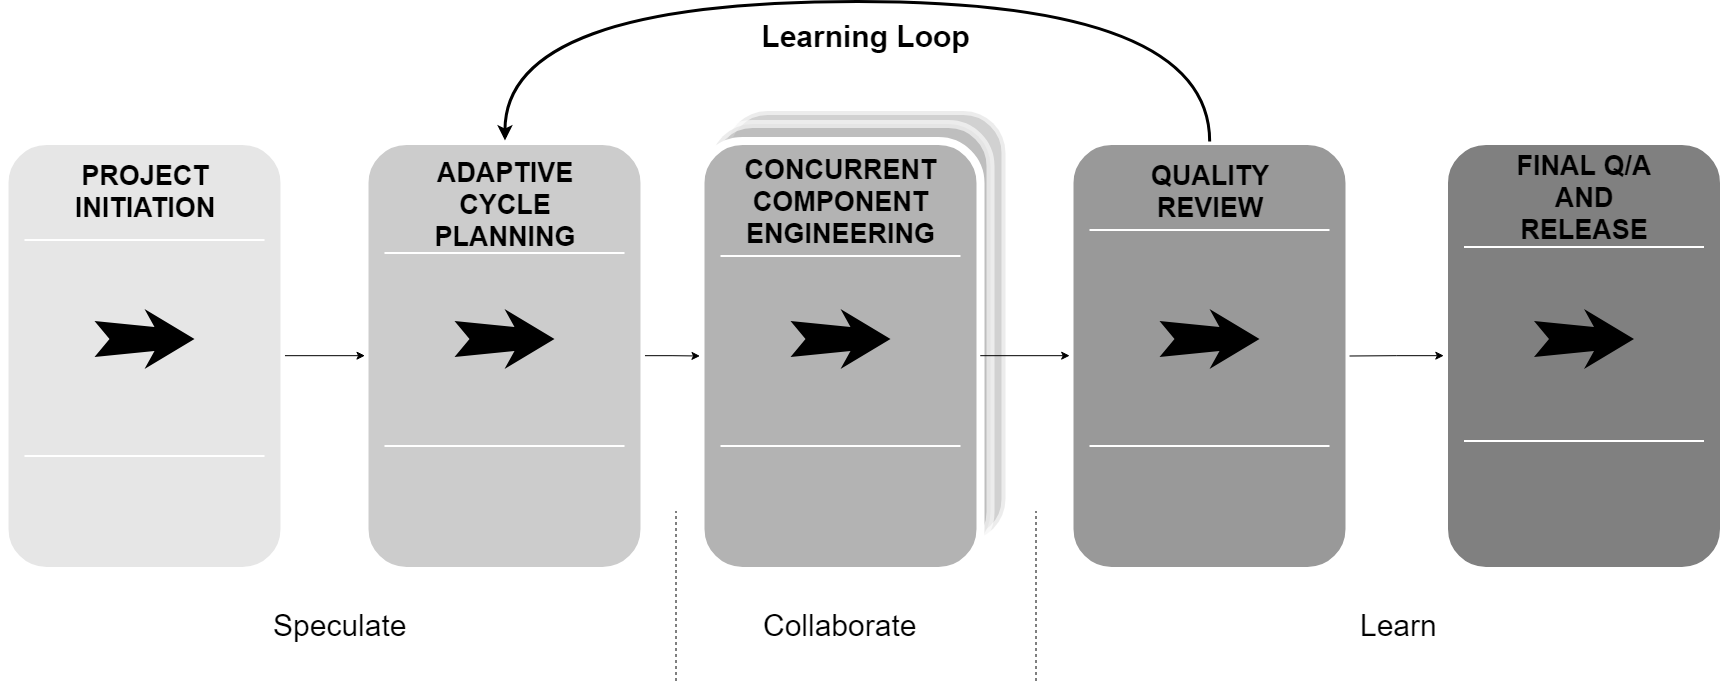
\includegraphics[scale=0.25]{figure/asd.png}
\caption{A redrawn illustration of the ASD model} %created by Jim Highsmith and Sam Bayer}
\label{asd}
\end{figure}

%%%%%
\begin{comment} 

% ----
% In the following sections, examples of a figure, an equation, a table, a chemical structure, a list, a listing and a to-do note are shown.

\section{Figure}
\begin{figure}[H]
\centering
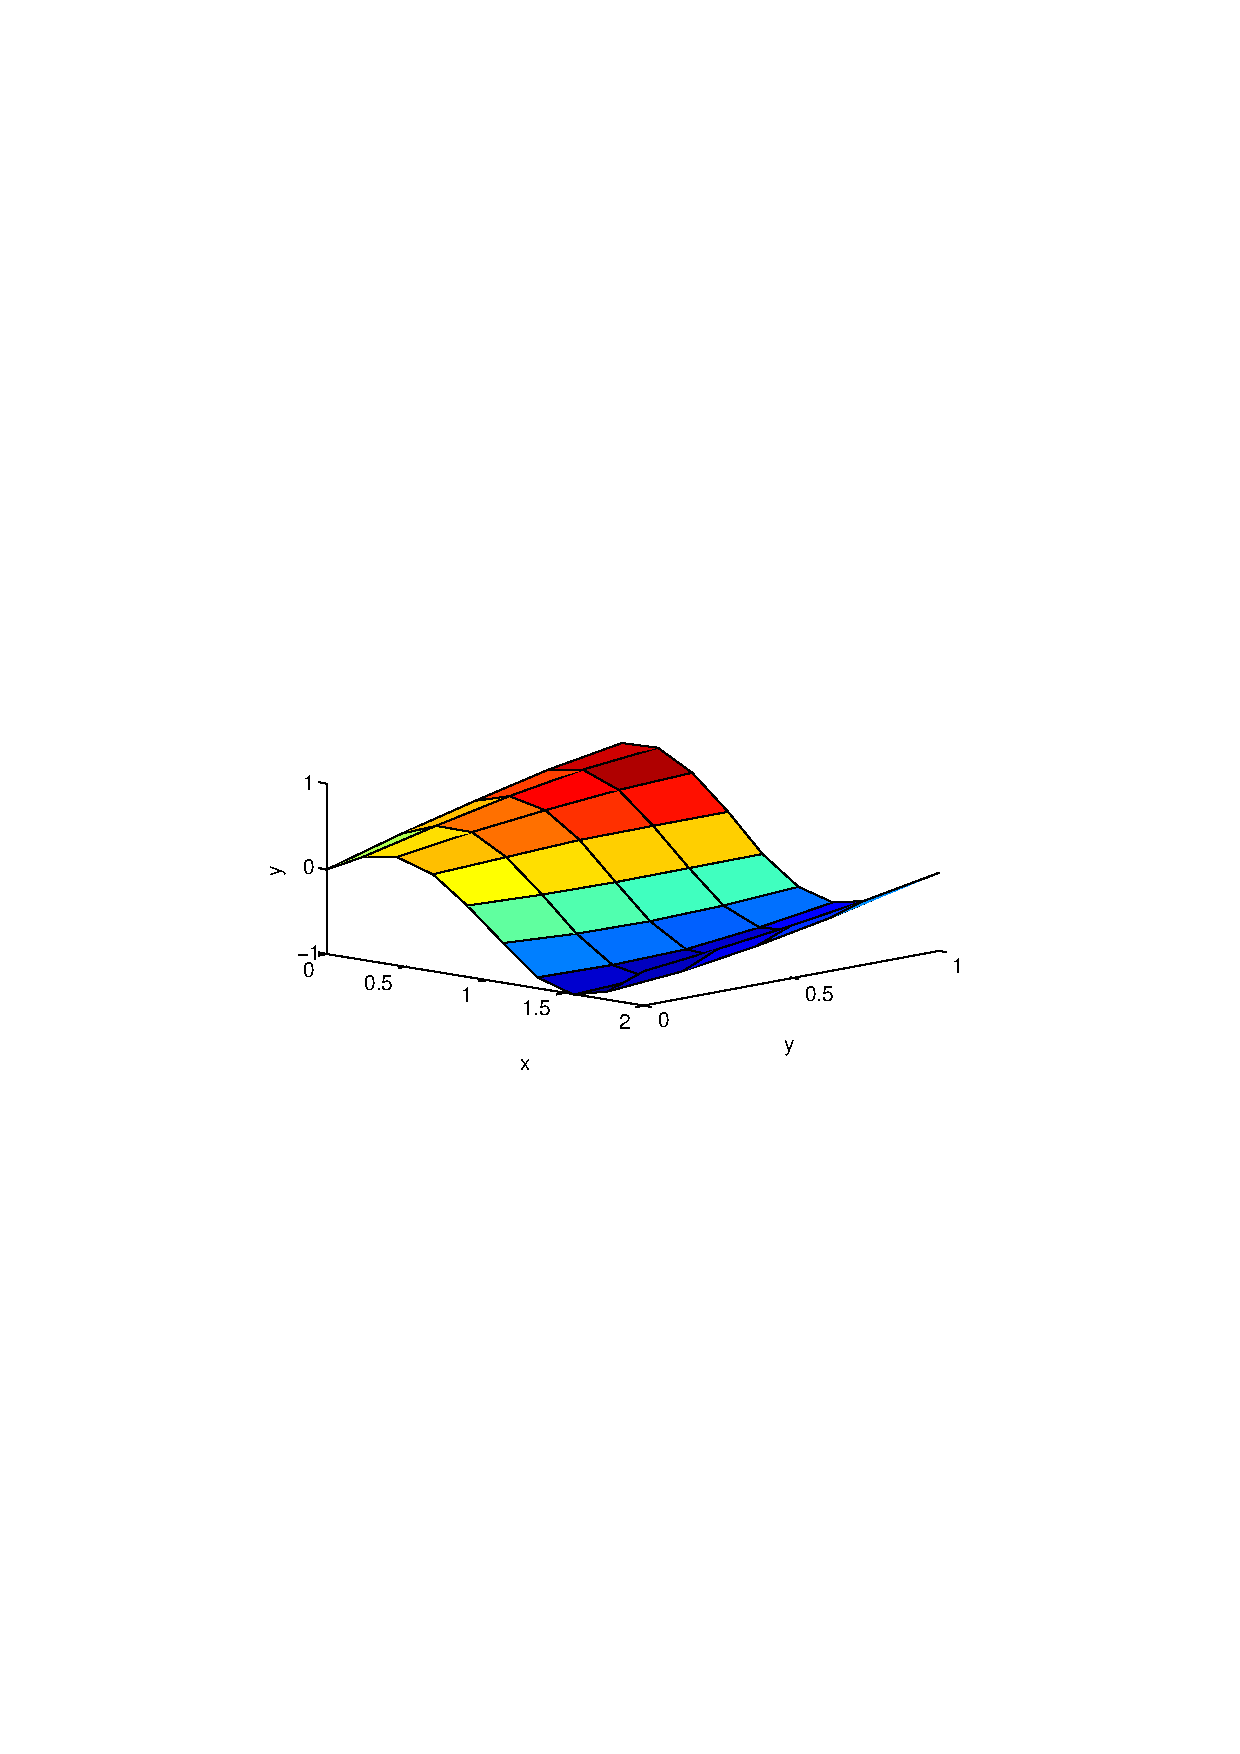
\includegraphics[width=0.45\linewidth, trim=3cm 11cm 3cm 11cm]{figure/X.pdf}
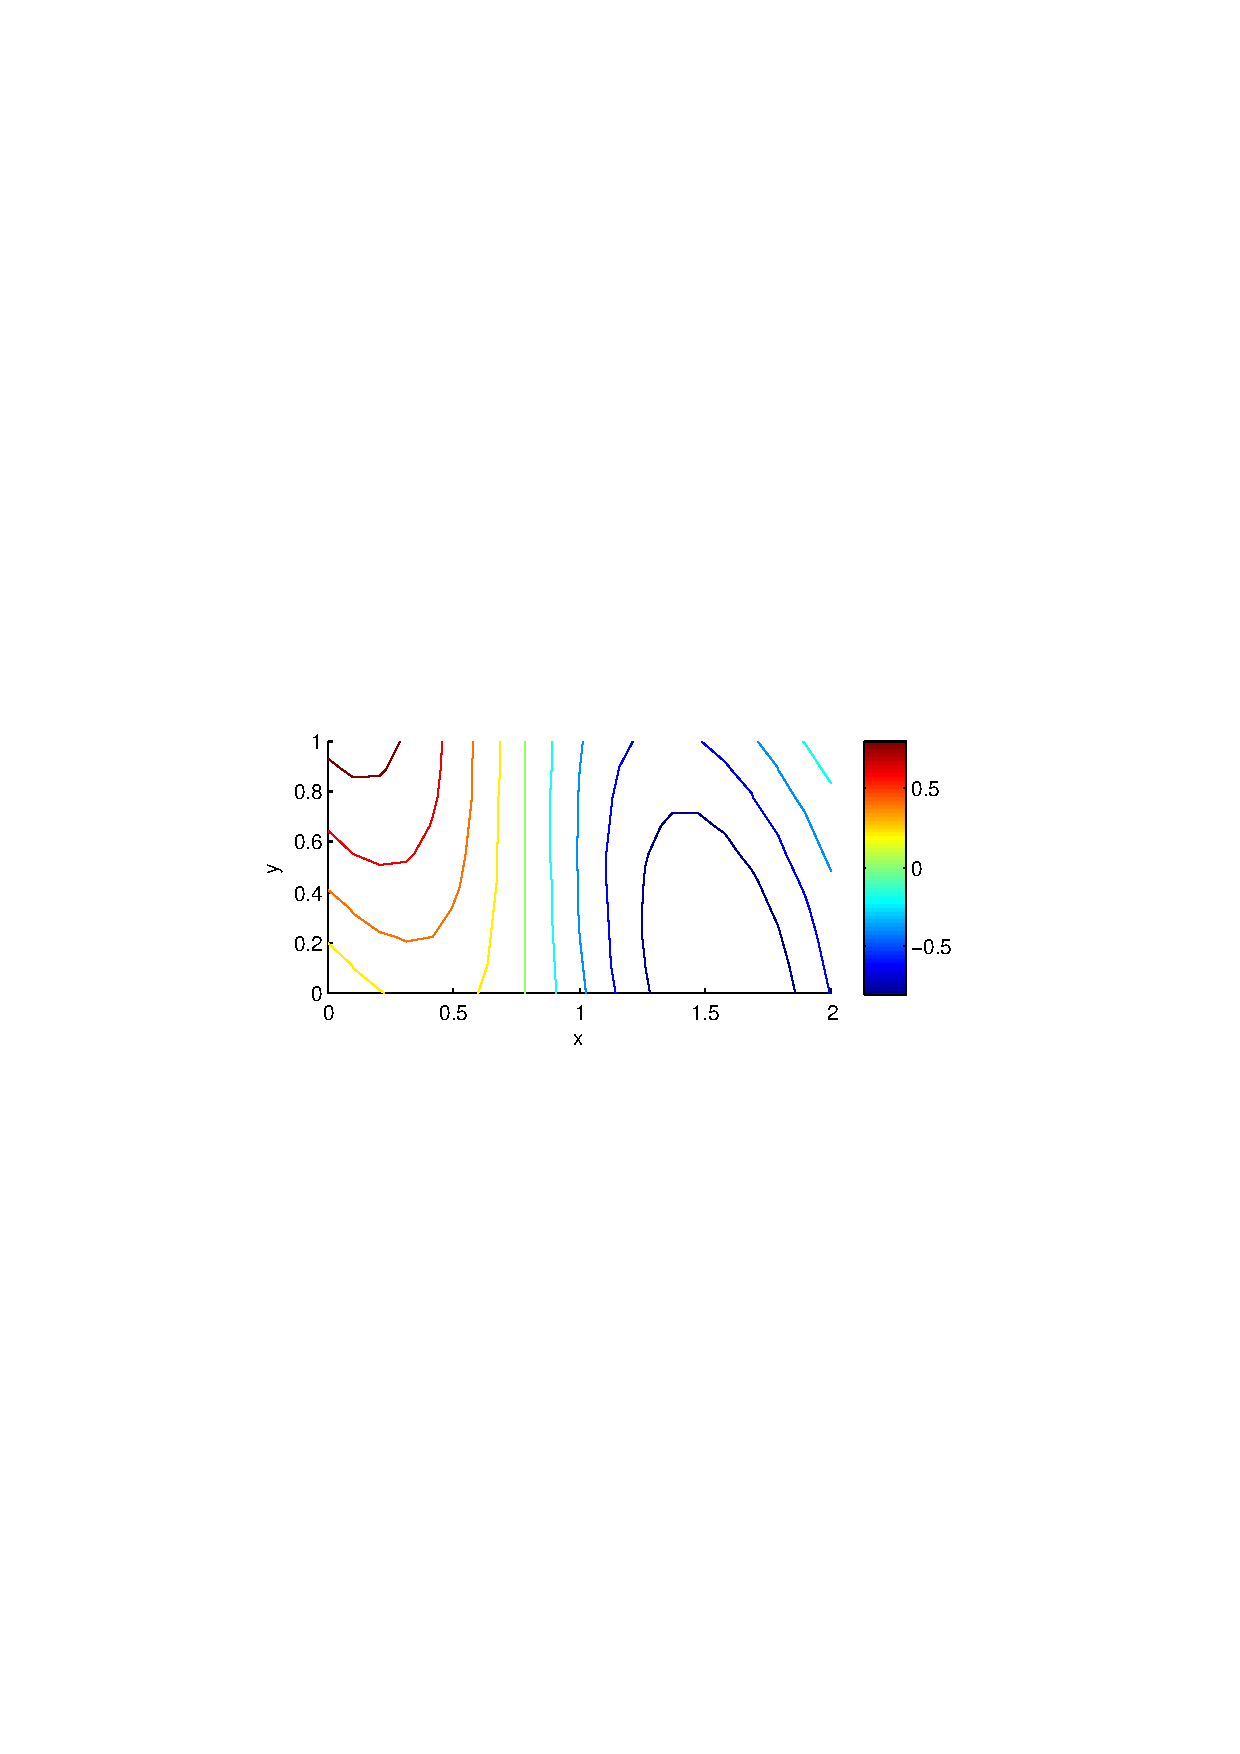
\includegraphics[width=0.45\linewidth, trim=3cm 11cm 3cm 11cm]{figure/Y.pdf}
\caption{Surface and contour plots showing the two dimensional function $z(x,y)=\sin(x+y)\cos(2x)$.}
\end{figure}

\section{Equation}
\begin{equation}
f(t)=\left\{ \begin{array}{ll}
1,~~~~ & t< 1 \\
t^2 & t\geq 1
\end{array}\right.
\end{equation}

\section{Table}
\begin{table}[H]
\centering
\caption{Values of $f(t)$ for $t=0,1,\dots 5$.}
\begin{tabular}{l|llllll} \hline\hline
$t$ & 0 & 1 & 2 & 3 & 4 & 5 \\ \hline
$f(t)$ & 1 & 1 & 4 & 9 & 16 & 25 \\ \hline\hline
\end{tabular}
\end{table}

\section{Chemical structure}
\begin{center}
\chemfig{X*5(-E-T-A-L-)}
\end{center}

\section{List}
\begin{enumerate}
  \item The first item
  \begin{enumerate}
    \item Nested item 1
    \item Nested item 2
  \end{enumerate}
  \item The second item
  \item The third item 
  \item \dots
\end{enumerate}

\section{Source code listing}
%\lstset{language=Matlab}
\begin{lstlisting}[frame=single]
% Generate x- and y-nodes
x=linspace(0,1); y=linspace(0,1);

% Calculate z=f(x,y)
for i=1:length(x)
 for j=1:length(y)
  z(i,j)=x(i)+2*y(j);
 end
end
\end{lstlisting}

\section{To-do note}
The \texttt{todo} package enables to-do notes to be added in the page margin. This can be a very convenient way of making notes in the document during the process of writing. All notes can be hidden by using the option \emph{disable} when loading the package in the settings. \todo{Example of a to-do note.}

\end{comment}
%%%%%